\chapter{Implementation}
In this chapter, details regarding the implementation of the samplers and the general setup of the artifical data used for evaluating the models are presented.
The Bayesian Markov Blanket and its SA extension were both implemented in Python 3 with the SciPy stack \citep{scipy}.
The code is openly available at
\begin{center}
	\href{https://github.com/FabricioArendTorres/BayesianMarkovBlanket/}{https://github.com/FabricioArendTorres/BayesianMarkovBlanket/}
\end{center}

\section{Sampling}
While SciPys statistics library includes many distributions to sample from,
more uncommon ones such as the GIG and MGIG are not covered.
Furthermore, SciPy relies on inverse transform sampling as a default sampling procedure,
which might not be optimal in terms of speed or numerical precision.
For the truncated normal distribution new sampling approaches have emerged that improve those aspects. 
As such they are preferable for the implementation of an MCMC sampler.
Last but not least, even for simple distributions such as the Normal distribution it can be beneficial to exploit the structure of the parameters for more efficient sampling procedures.
In this section we will expand on the methods used for sampling from the respective distributions in the presented Gibbs sampler.

\subsection{Normal Distribution: $\Wxy$}
\label{W12_draw}
We want to draw samples from:
\begin{align*}
	\text{vec}(\matr{W}_{12}) | \matr{W}_{11}, \matr{T}, \matr{S}, \lambda & \sim \mathcal{N}(-\matr{C}^{-1} \text{vec}(\matr{S}_{12}), \matr{C}^{-1}) 
	\\
	\matr{C} = \Big[
	(\matr{S}_{22} + \matr{I})                                             & \otimes \matr{W}_{11}^{-1} +\matr{D}\Big]                                 
\end{align*}

A naive approach would require the inversion of $\matr{C}$, a $(pq)\times(pq)$ matrix, where $q$ is known to be rather large.
This should be avoided, as the inversion is computationally expensive.

Instead we can sample from the transpose using Theorem \autoref{th:231}.
\begin{tcolorbox}[colback=yellow!5!white,colframe=yellow!75!black]
	\begin{customthm}{2.3.1}[\cite{gupta2018matrix}, Chapter 2.3]
		\label{th:231}
		If $\matr{X} \sim \mathcal{N}_{p,n}(\matr{M}, \matr{\Sigma} \otimes \matr{\Psi})$ then $\matr{X}^T \sim \mathcal{N}_{n,p}(\matr{M}^T, \matr{\Psi} \otimes \matr{\Sigma})$
	\end{customthm}
\end{tcolorbox}

This leads to:
\begin{tcolorbox}[colback=red!5!white,colframe=red!60!black]
	\begin{align*}
		\text{vec}(\matr{W}_{12}^T) | \matr{W}_{11}, \matr{T}, \matr{S}, \lambda & \sim \mathcal{N}(-(\matr{C'})^{-1} \text{vec}(\matr{S}_{12}^T), (\matr{C'})^{-1}) 
		\\
		\matr{C'} = \Big[
		\matr{W}_{11}^{-1}                                                       & \otimes (\matr{S}_{22} + \matr{I})+\matr{D}\Big]                                  
	\end{align*}
\end{tcolorbox}
where $\matr{C}'$ now admits a block-wise structure that can be exploited for an efficient Cholesky decomposition (as shown by \citet{kaufmann_bayesian_2015}).

Let $\matr{Q}=\Wxx^{-1}$
and $\matr{D} = \text{diag}(\matr{D}_1,\dots,\matr{D}_p)$.
then:
\[
	\matr{C}'=
	\begin{bmatrix}
		Q_{11}(\Syy+\matr{I})+\matr{D}_1 & \dots & Q_{1j}(\Syy+\matr{I}) & \dots & Q_{1p}(\Syy+\matr{I})              \\
		\vdots                           &       &                       &       & \vdots                             \\
		Q_{i1}(\Syy+\matr{I})            &       & \ddots                &       & Q_{ip}(\Syy+\matr{I})              \\
		\vdots                           &       &                       &       & \vdots                             \\
		Q_{p1}(\Syy+\matr{I})            & \dots & Q_{pj}(\Syy+\matr{I}) & \dots & Q_{pp}(\Syy+\matr{I}) + \matr{D}_p 
	\end{bmatrix}
\]

A block-wise Cholesky decomposition of the form
$$
\matr{C}' = \matr{L} \matr{L}^T
$$
is then given by

\newcommand{\syyi}{(\Syy + \matr{I})}
\newcommand{\blockunw}[1]{\Big(Q_{#1#1}\syyi+\matr{D}_#1\Big)}
\[
	\matr{L}^T=
	\begin{bmatrix}
		\matr{K}_1^\frac{1}{2} & Q_{12} \matr{B}_1      & \cdots & Q_{1j} \matr{B}_1      & \cdots & Q_{1p} \matr{B}_1      \\
		\matr{0}               & \matr{K}_2^\frac{1}{2} & \cdots & Q_{2j} \matr{B}_2      & \cdots & Q_{2p} \matr{B}_2      \\
		\vdots                 & \vdots                 & \ddots & \vdots                 &        & \vdots                 \\
		\matr{0}               & \matr{0}               & \cdots & \matr{K}_j^\frac{1}{2} & \cdots & Q_{jp} \matr{B}_j      \\
		\vdots                 & \vdots                 &        & \vdots                 & \ddots & \vdots                 \\
		\matr{0}               & \matr{0}               & \cdots & \matr{0}               & \cdots & \matr{K}_p^\frac{1}{2} 
	\end{bmatrix}
\]
with
\begin{align*}
	\matr{K}_i & = \blockunw{i}                   
	\\
	\matr{B}_i & = \matr{K}_i^{-\frac{1}{2}}\syyi 
\end{align*}

Non-diagonal entries only differ by a (scalar) factor $Q_{ij}$, which allows for an efficient computation by reusing the $\matr{B}_i$.
The $\matr{K}_i^{\frac{1}{2}}$ can be calculated by a naive Cholesky decomposition as $\matr{K}_i$ are symmetric positive definite.

For drawing from the Normal distribution we can simply draw from a standard Normal Distribution and then transform it by multiplying with the standard deviation and adding the mean \cite[Chapter 7.4]{gentle2009computational}.
In our context this corresponds to Algorithm \autoref{alg:MN_sampler},
where the mean and standard deviation are calculated from the above mentioned block-wise Cholesky decomposition.



\begin{algorithm}[]
	\caption{Draw Sample from $\mathcal{N}\big(-(\matr{C'})^{-1} \text{vec}(\matr{S}_{12}^T), \matr{C'}^{-1}\big)$}\label{alg:MN_sampler}
	\begin{algorithmic}
		\Function{draw\_W12}{$\Wxx, \Syy, \matr{D}$}
		\\
		\State Compute $\matr{L} \gets BlockChol(\Wxx^{-1}, \Syy, \matr{D})$
		\\
		\State Solve for $y$: $\qquad \matr{L}y=-\text{vec}(\Sxy^T) $ 
		\Comment{using forward substitution}
		\State Solve for $\mu$: $\qquad \matr{L}^T\mu=y$
		\Comment{using backward substitution}
		\\
		\State Sample $\qquad\quad\ \  r \sim \mathcal{N}(0,\matr{I}_{pq})$
		\State Solve for $b$: $\qquad \matr{L}^T b=r$
		\Comment{using backward substitution}
		%		\\
		\State
		\Return $(b+\mu)$
		\Comment{$(b+\mu)\sim \mathcal{N}\big( -(\matr{C'})^{-1} \text{vec}(\matr{S}_{12}^T), \matr{C'}^{-1}\big)$}
		\EndFunction
	\end{algorithmic}
\end{algorithm}


\subsection{Matrix Generalized Inverse Gaussian: $\Wxx$}
\label{sample_MGIG}
For the $\Wxx$ block we have to sample from
$$
\matr{W}_{11} | \matr{W}_{12}, \matr{T}, \matr{S}, \lambda \sim 
\mathcal{MGIG}_B
\Big(
\lambda' = \frac{n+p+1}{2}, \ 
\matr{A} = \matr{S}_{11}+\matr{I},\  
\matr{B} = \matr{W}_{12}(\matr{S}_{22}+I)\matr{W}_{12}^T
\Big)
$$
\citet{bernadac_random_1995} has shown that the \gls{MGIG} can be represented as a continued fraction of Wishart random variables.  
Similar to \citet{kaufmann2017semi} we make use of this result for the sampling process.
\begin{tcolorbox}[colback=yellow!5!white,colframe=yellow!75!black]
	\begin{theorem_51but}
		Let $\matr{X}, \matr{Y}_1, \matr{Y}_2$ be independent random variables,
		\\
		such that
		$$
		\mathcal{L}(\matr{Y}_1) = \mathcal{W}_p(2k, \matr{B'}^{-1})
		\quad \quad
		\mathcal{L}(\matr{Y}_2) = \mathcal{W}_p(2k, \matr{A'}^{-1})
		\quad \quad
		k > \frac{p-1}{2}
		$$
		$$
		\mathcal{L}(\matr{X}) = \mathcal{MGIG}_B\big(-k, \matr{A'}, \matr{B'} \big)
		$$
		$$
		\text{iff} \quad \mathcal{L}(\matr{X}) = \mathcal{L}((\matr{Y}_1 + (\matr{Y}_2 + \matr{X})^{-1})^{-1})
		$$
	\end{theorem_51but}
\end{tcolorbox}
However, the condition for $\lambda'$ does not hold in our given MGIG distribution:
$$
k = -\frac{n+p+1}{2} < \frac{p-1}{2} \qquad \text{\Lightning}
$$

It is important to note at this point, that the relation between the degrees of freedom $-\lambda' = 2df$ arises from comparing the determinant of the Wishart to the determinant of the MGIG reparameterized by its inverse in \autoref{propos_34}.
\begin{tcolorbox}[colback=yellow!5!white,colframe=yellow!75!black]
	\begin{propos_34but}
		\begin{equation}
			\label{propos_34}
			\mathcal{L}(\matr{X}) = \mathcal{MGIG}_B(\lambda', \matr{A}', \matr{B}') 
			\Leftrightarrow 
			\mathcal{L}(\matr{X}^{-1}) = \mathcal{MGIG}_B(-\lambda', \matr{B}', \matr{A}')
		\end{equation}
	\end{propos_34but}
\end{tcolorbox}

For addressing the constraint issue, the MGIG is written in terms of the parameterization by Letac (similar to the \gls{GIG} formulation in \cite{letac1983characterization}):
\begin{equation*}
	\matr{X} \sim \mathcal{MGIG}_{L}(n', \matr{A}, \matr{B}) 
\end{equation*}
\begin{equation}
	\label{eq:MGIG_L}
	p(\matr{X}) \propto \det(\matr{X})^{-n' - 1}
	\exp \tr
	\Big(
	-\frac{1}{2} (\matr{A}\matr{X} + \matr{B} \matr{X}^{-1} )
	\Big)
\end{equation}
with the condition now being \cite[Appendix 4]{kaufmann2017semi}:
$$
n'>\frac{p-1}{2}
$$
A change of variable to its inverse with $\matr{W}=\matr{X}^{-1}$ with Jacobian $det(\matr{W})^{-(p+1)}$ 
leads to:
\begin{align}
	p(\matr{W}) & \propto \det(\matr{W}^{-1})^{-n' - 1} 
	\exp \tr
	\Big(
	-\frac{1}{2} (\matr{A}\matr{W}^{-1} + \matr{B} \matr{W} )
	\Big)
	\nonumber
	\\
	            & = \det(\matr{W})^{n'-p}               
	\exp \tr
	\Big(
	-\frac{1}{2} (\matr{A}\matr{W}^{-1} + \matr{B} \matr{W} )
	\Big)
	\label{eq:inverse_MGIG}
\end{align}
If the posterior conditional is now expressed in terms of \autoref{eq:inverse_MGIG},
the corresponding inverse formulated as in \autoref{eq:MGIG_L} fulfills the constraint
and we can sample from this inverse.

With the posterior conditional being (see \autoref{A:post_cond} for details)
\[
	p(\matr{W}_{11} | \matr{W}_{12}, \matr{T}, \matr{S}, \lambda)
	\propto
	\det(\matr{W}_{11})^{n/2}
	\exp \Big(
	-\frac{1}{2} \tr\big[
		(\matr{S}_{11}+ \matr{I})\matr{W}_{11} + \matr{W}_{12}(\matr{S}_{22}+\matr{I})\matr{W}_{12}^T \matr{W}_{11}^{-1}
	\big]
	\Big)
\]
a comparison with \autoref{eq:inverse_MGIG} gives
\begin{align*}
	A              & =  \matr{W}_{12}(\matr{S}_{22}+\matr{I})\matr{W}_{12}^T 
	\\
	B              & = \matr{S}_{11}+ \matr{I}                               
	\\
	\frac{n}{2}    & = n'-p                                                  \\
	\Rightarrow n' & = \frac{n}{2}+p                                         
\end{align*}
So the inverse of our posterior conditional is
$$
\matr{W}_{11}^{-1} | \matr{W}_{12}, \matr{T}, \matr{S}, \lambda \sim \mathcal{MGIG}_L\Big(n'=\frac{n}{2}+p, A=(\matr{W}_{12}(\matr{S}_{22}+\matr{I})\matr{W}_{12}^T), B=(\matr{S}_{11}+ \matr{I}) \Big)
$$
For this inverse, the required constraint is satisfied:
$$
n' = \frac{n}{2}+p > \frac{(p-1)}{2}
$$

For sampling from the inverse, the determinant of this \gls{MGIG} is compared to the determinant of the Wishart distribution.
\begin{align*}
	n'-1=\frac{n}{2}+p-1 & = \frac{df-p-1}{2} 
	\\
	\Rightarrow df       & = n+3p-1           
\end{align*}
Finally, a sample can be drawn by the following continued fraction
$$
X = \Big((Y_1)_1 + 
\Big((Y_2)_1 + 
\Big( (Y_1)_2 + 
\Big( (Y_2)_2 + \dots \Big)^{-1} 
\Big)^{-1} 
\Big)^{-1}
\Big)^{-1}
$$
$$
(\matr{Y}_1)_i 
\sim 
\mathcal{W}_p
\Big(
n+3p-1, 
(\Wxy(\matr{S}_{22}+\matr{I})\Wxy^T)^{-1}
\Big)
\quad \quad
(\matr{Y}_2)_i 
\sim 
\mathcal{W}_p 
\Big(
n+3p-1, 
(\matr{S}_{11}+\matr{I})^{-1}
\Big)
$$
and then inverting the result:
$$
\Wxx = {X}^{-1}
$$

As we are drawing the inverse of the r.v. we are interested in, simply omitting the last inversion in the continued fraction leads to the desired result.
\subsubsection*{Simulated Annealing}
In case of the Simulated Annealing, the cooled posterior conditional is 
\[
	p(\matr{W}_{11} | \matr{W}_{12}, \matr{T}, \matr{S}, \lambda)^{1/\Tc}
	\propto
	\det(\matr{W}_{11})^{n/(2\Tc)}
	\exp \Bigg(
	-\frac{1}{2} \tr\Big[
		\frac{(\matr{S}_{11}+ \matr{I})}{\Tc}\matr{W}_{11} + \frac{\matr{W}_{12}(\matr{S}_{22}+\matr{I})\matr{W}_{12}^T}{\Tc} \matr{W}_{11}^{-1}
	\Big]
	\Bigg)
\]
Consequently the comparison with the inverted MGIG in \autoref{eq:inverse_MGIG} is slightly different:
\begin{align*}
	A              & =  \frac{\matr{W}_{12}(\matr{S}_{22}+\matr{I})\matr{W}_{12}^T }{\Tc} 
	\\
	B              & = \frac{\matr{S}_{11}+ \matr{I}}{\Tc}                                
	\\
	\frac{n}{2\Tc} & = n'-p                                                               \\
	\Rightarrow n' & = \frac{n}{2\Tc}+p                                                   
\end{align*}
Note, that the constraint is still satisfied for any $\Tc>0$:
$$
n' = \frac{n}{2\Tc}+p > \frac{(p-1)}{2}
$$
Comparing the determinant with the Wishart:
\begin{align*}
	n'-1=\frac{n}{2\Tc}+p-1 & = \frac{df-p-1}{2}   
	\\
	\Rightarrow df          & = \frac{n}{\Tc}+3p-1 
\end{align*}
Finally, a sample can be drawn by the following continued fraction
$$
X = \Big((Y_1)_1 + 
\Big((Y_2)_1 + 
\Big( (Y_1)_2 + 
\Big( (Y_2)_2 + \dots \Big)^{-1} 
\Big)^{-1} 
\Big)^{-1}
\Big)^{-1}
$$
$$
(\matr{Y}_1)_i 
\sim 
\mathcal{W}_p
\Bigg(
\frac{n}{\Tc}+3p-1, 
\Big(
\frac{\matr{W}_{12}(\matr{S}_{22}+\matr{I})\matr{W}_{12}^T }{\Tc}
\Big)^{-1}
\Bigg)
\quad \quad
(\matr{Y}_2)_i 
\sim 
\mathcal{W}_p 
\Bigg(
\frac{n}{\Tc}+3p-1, 
\Big(
\frac{\Sxx+ \matr{I}}{\Tc}
\Big)^{-1}
\Bigg)
$$
and then inverting the result:
$$
\Wxx = {X}^{-1}
$$
\subsection{Truncated Normal Distribution}
The inverse transform sampling implemented in SciPy fails and returns infinity for bounds that are far away from the mean.
Dependent on the data, this can break the copula Gibbs sampler, so an alternative method is required.
In the original implementation of the BMB by \citet{kaufmann_bayesian_2015}, the rejection sampler by \citet{geweke1991efficient} was used.
We follow a more recent approach presented by \citet{chopin2011fast}.
Compared to the rejection sampler, it offers slightly higher precision and speed.
Furthermore it does not require a table setup for sampling values from a new set of parameters.
In context of the copula, this is obviously a useful property as the scores are sampled from a new set of parameters each iteration.

\subsection{Generalized Inverse Gaussian}
For the GIG we utilize the sampler of the R package \textit{GIGrvg}
\footnote{\href{https://cran.r-project.org/web/packages/GIGrvg/}{https://cran.r-project.org/web/packages/GIGrvg/}}.
It is based on three different algorithms, each of which has performance advantages for specific ranges of the parameter values. 
The algorithms have been introduced by \citet{hormann2014generating} and \citet{lehner1989erzeugung} (which is a version of \citet{dagpunar1989easily} with a faster setup).

Alternative approaches may be faster for sampling multiple values from fixed parameters, but require a much longer setup. 
As mentioned before, this is disadvantageous in our setting.

The code was included by wrapping a C++ implementation\footnote{\href{https://github.com/horta/gig}{https://github.com/horta/gig}} of the R code in Cython. It is openly available via
\begin{center}
	\href{https://github.com/FabricioArendTorres/gig}{https://github.com/FabricioArendTorres/gig}
\end{center}

\section{Artificial Data: Setup and Metrics}
For evaluating the performance of the different network reconstruction methods, a data set that reflect the properties of the networks encountered in real applications is required.

We base the creation of the artificial data on the setup of \citet{kaufmann_bayesian_2015},
which will be described in the subsequent section.
For measuring how well the networks are reconstructed, a simple approach based on counting correctly predicted edges is followed.

\subsection{Data Setup}
\label{subs:artdata}

Each artificial data set is created by drawing 1000 samples from a zero-mean normal distribution 
$
\mathcal{N}_{p+q}(\matr{0}, \W^{-1})
$
with $p=10$ and $q=90$.
The structure of $\W$ is created according to a beta-binomial model.
That is, we first draw from the beta distribution
$$
\matr{\pi}_i \sim Beta(\alpha=0.01, \beta=1) \qquad i=1,\dots,(p+q)
$$
and then use the $\pi$ for drawing from a binomial
$$
{n}_{ij} \sim Bin(n=1, p=\pi_i) \qquad j = 1, \dots,(p+q)
$$
where ${n}_{ij}=1$ indicates that $\W_{ij}$ is non-zero and vice-versa.
As $E[\pi] = \frac{\alpha }{(\alpha+\beta)} = \frac{1}{101}$, the resulting network will be mostly sparse (i.e. have few edges) with only few nodes having a high $\pi$.
The few that have a higher $\pi$ will then exhibit a lot of edges to other nodes, resulting in a small-world structure of the network.

This sampling process can be repeated until a neighborhood structure fulfilling specific requirements is created.
In our case, those requirements are limits for the number of neighbors in $\Wxy$ and $\Wyy$:
\begin{enumerate}
	\item $5p < \sum\limits_{i=1}^{p} \sum\limits_{j=p+1}^{p+q}{n}_{ij} < q$
	\item $q < \sum\limits_{i=p+1}^{p+q} \sum\limits_{j=p+1}^{p+q}{n}_{ij} < 2q$
\end{enumerate}
The first requirement implies, that the fraction of non-zero edges lies between $\frac{5p}{pq}$ and $\frac{1}{p}$.
For $p=10$ and $q=10$ this means that $90\%$ to $94.\overline{4}\%$ of the edges in $\Wxy$ are zero. 

Finally, the edge weights are calculated by drawing uniformly from $[0.3,1]$ and then randomly flipping the sign of the weight:
\begin{align*}
	        & w_{ij} \sim \mathcal{U}(0.3, 1) \\
	        & f_{ij} \sim \mathcal{U}(-1,1)   
	\\
	\W_{ij} & = {n}_{ij} * w_{ij}  * sgn(f)   
\end{align*}

The resulting networks exhibits many connections to a few selected nodes, similarly to the real-world problems we target.
An example network is shown in \autoref{fig:example_newtork}.

\begin{figure}[H]
	\centering
	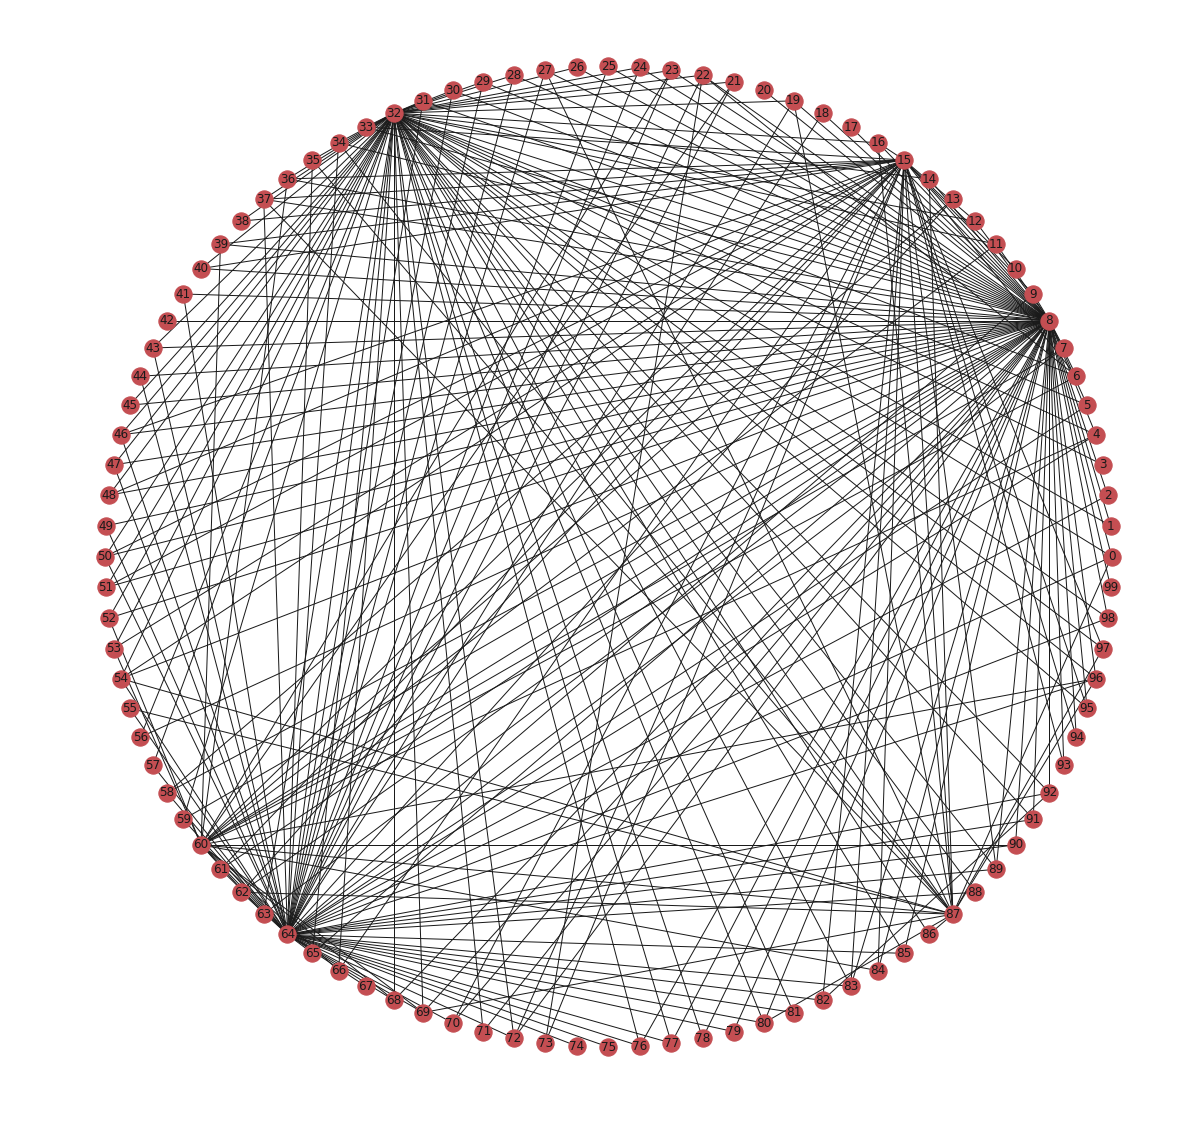
\includegraphics[width=0.48\textwidth]{data_fullgraph.png}
	\caption{Example network for $p=10$ and $q=90$, ordered such that the first $10$ nodes correspond to $p$. It can be seen that the network exhibits small-world properties in form of a few highly connected nodes, both in the $p$ as well as in the $q$ variables.}
		
	\label{fig:example_newtork}
\end{figure}

\subsection{Performance Metrics}
The metrics used for measuring the performance should be focused on how the structure of the predicted network graph compares to the ground truth.
But the problem of quantifying dissimilarities between graphs is in itself a difficult and computationally expensive one.
Instead we follow the simple approach of counting the prediction errors.
Similarly to \cite{kaufmann_bayesian_2015}, prediction of an (existing) edge with the wrong sign is counted as a false positive, as shown in the following confusion matrix.
\begin{table}[H]
	\centering
	\resizebox{0.8\textwidth}{!}{%
		\begin{tabular}{cccccc}
			&&&\multicolumn{3}{c}{\textbf{Actual}} 
			\\
			  &                  &   & $(\Wxy)_{i,j}<0$ & $(\Wxy)_{i,j}>0$ & $(\Wxy)_{i,j}=0$ 
			\\
			%\cmidrule{4-5}
			\multirow{3}{*}{\textbf{Predicted}}
			  & $(\Wxy)_{i,j}<0$ &   & TP               & FP               & FP               \\
			  & $(\Wxy)_{i,j}>0$ &   & FP               & TP               & FP               \\
			  & $(\Wxy)_{i,j}=0$ &   & FN               & FN               & TN               
		\end{tabular}}
\end{table}
On this basis, commonly known metrics such as the sensitivity (recall), specificity and precision can be calculated:

\begin{align*}
	sensitivity & = \frac{TP}{TP+FN} \\
	specificity & = \frac{TN}{TN+FP} \\
	precision   & = \frac{TP}{TP+FP} 
\end{align*}

As there is always a trade-off between these, we also look at the F-score and the Matthews correlation coefficient.
The F score is the harmonic mean between precision and recall, while the MCC is a measure of correlation between the predicted and the actual values \citep{baldi2000assessing}.

\[
	F = \frac{2TP}{2TP + FP + FN}
\]\\
\[
	MCC = \frac{TP \times TN - FP \times FN}{\sqrt{(TP + FP) (TP + FN) (TN+FP) (TN+FN)}}
\]

